\chapter{Développements}
\label{chap:developpements}

Ce chapitre expose les modifications faites dans le logiciel Proteus et dans X-plor pendant la préparation de cette thèse.

X-plor est un logiciel concue pour la biologie struturale et developpé à l'origine par Axel T. Brünger à l'université de Yale , \cite{Brünger92}. Il propose un language de script permettant d'exploiter ses Pour adapter X-plor au CPD nous y ajoutons la gestion de jeux de coordonnées multiples pour chaque résidu.

Le REMC est par nature un algorthme parallèle, nous présentons l'implementation de cet algorithme dans proteus avec notre gestion du parallèlisme. Le schéma proposé par et Metropolis et Hasting constitue un cadre général dans lequel il est possible d'apadpter les probabilités utilisées au système étudier. Nous expliquons comment le critère d'acceptation a été amélioré en tenant compte de la spécificité de notre modèle et de nos objectifs. Enfin, sont présenté quelques nouvelles fonctionnalité dans proteus.  


\section{Les Modèles }

Proteus , lors de la préparation du système, place chaque chaîne latérale possible aux différentes positions de la chaîne polypeptidique selon la librairie de rotamère de Tufery. Ces placements sont utilisés à de nombreuses reprises pendant le calcul des énergies d'interactions. X-plor ne permettait qu'une gestion de quatres jeux de coordonnées pour une chaîne latérale simulatement. Cela oblige l'utilisaton de nombreux fichiers qui stockent les jeux de coordonnées.

Afin de remédier à ce problème, nous modifions le code source d'X-plor pour y introduite deux nouvelles notions. Une resclass identifie un résidu par un triplet composé du resid , du resname et du segid. Ces trois notions, existantes dans le format PDB et X-plor, représentent respectivement la position dans une chaîne polypeptidique , le type d'acide aliné, la chaîne. Un modèle est un jeu de coordonnées d'une resclass. Une resclass peut avoir plusieurs modèles.


   \begin{figure}[!htbp]
     \centering
     \begin{tabular}{c}
       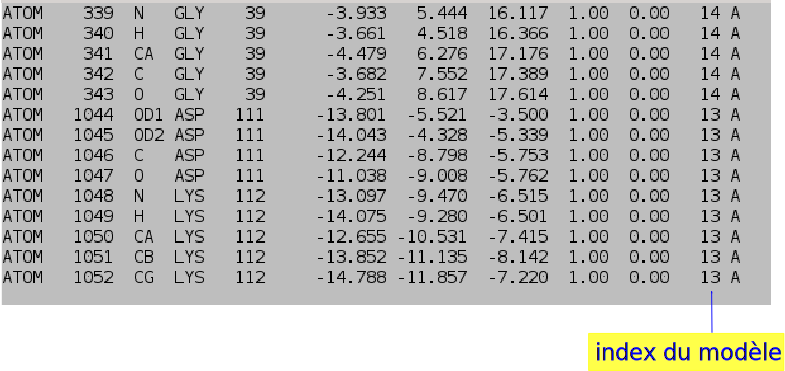
\includegraphics[width=12cm]{figure/PDB.png} 
     \end{tabular}     
     \caption{\textbt{}}
\label{fig:PDB}
   \end{figure}


L'utilisateur ne manipule que les modèles; les resclass n'apparaissent ni dans les fichiers d'entrée/sortie ni dans les commandes. Un modèle se déclare par des lignes ATOM d'un fichier PDB. 
Il y a deux possiblités de lecture des modèles.

La commande:

\verb!coor disp=model @file.pdb!

ajoute chaque modèle de file.pdb dans un tableau en mémoire, Un nombre est lu à la colonne 67-71, Il représente l'indice du modèle pour une resclass. Le lien avec la resclass se fait via la listes des atomes contenant l'indice, voir une exemple à la figure \ref{fig:PDB}.

La commande:

\verb!coor disp=model @file.pdb push=true!

ajoute un seul modèle par resclass. L'indice d'un modèle n'est pas lu mais calculé comme le plus grand indice plus un. 

La copie de modèle se fait par la commande:

\verb!coor copy from=A to=B idx=i=j end!

avec \verb!A! et \verb!B!  pouvant prendre les valeurs \verb!main!, \verb!comp!, \verb!xref! ou \verb!model!.

Le mot \verb!idx=i=j! n'est pas obligatoire. Par défaut, si \verb!from=model! alors \verb!idx=1! et si \verb!to=model!  le nouvel indice créé sera le plus grand indice plus un.

L'ancienne syntaxe est toujours supportée.

La commande 

\verb!write coor sele=(resid $1 and resn $aa1) from=model output=new.pdb end!

imprime les modèles de chaque resclass défini par la sélection dans un fichier PDB. C'est-à-dire écrit une ligne par atome de la resclass avec l'indice du modèle, pour tous les modèles. 

Il est possible de limiter l'impression au modèle i par une commande du type:

\verb!write coor from=model idx=i output=new.pdb end!


\section{OpenMP pour le REMC}
\subsection{présentation d' OpenMP}

Pour l'implementation du \og Replica Exchange Monte Carlo\fg nous devons parallèliser la partie Monte-Carlo de proteus. Comme à ce stade, la matrice d'énergie parallèle n'est pas envisagée nous nous orientons vers une programmation à mémoire partagé. Dans ce domaine, l'interface de programmation OpenMP pour \og Open Multi-Processing\fg  offre un standard mature, bien supporté par les compilateurs C/C++, Fortran et simple à mettre en oeuvre. Il s'agît d'une spécification qui décrit une collection de directives au compilateur, une bibliothèques de routines et un ensembles de variables d'environnement. 


Le principe est d'ajouter à un code existant des directives pour définir:

\begin{itemize}
\item les instructions à exécuter en parallèle (création de fils d'exécution)
\item les situations de synchronisations entre fils d'exécution
\item le status des variables (partagé entre fils, privé,etc) 
\end{itemize}

La bibliothèque OpenMP permet la configuration de l'exécution et son contrôle par un ensemble de fonctons et de macros. Il existe des fonctions qui gèrent le nombre de fils d'exécutioin, qui fixent la politique de l'ordonnancement, qui retourne un identifiant du fils d'exécution, etc. La définition de la macro \_OPENMP garantie la compatibilité de l'éxécutable.
Les variables d'environnement contrôle les mêmes informations que les fonctions openMP et doivent définis avant l'éxecution. Elles sont prises en compte avec une priorité plus faible que les fonctions de la bibliothèque elles-mêmes de priorité plus faible que les directives en cas de conflit.

   \begin{figure}[!htbp]
     \centering
     \begin{tabular}{c}
       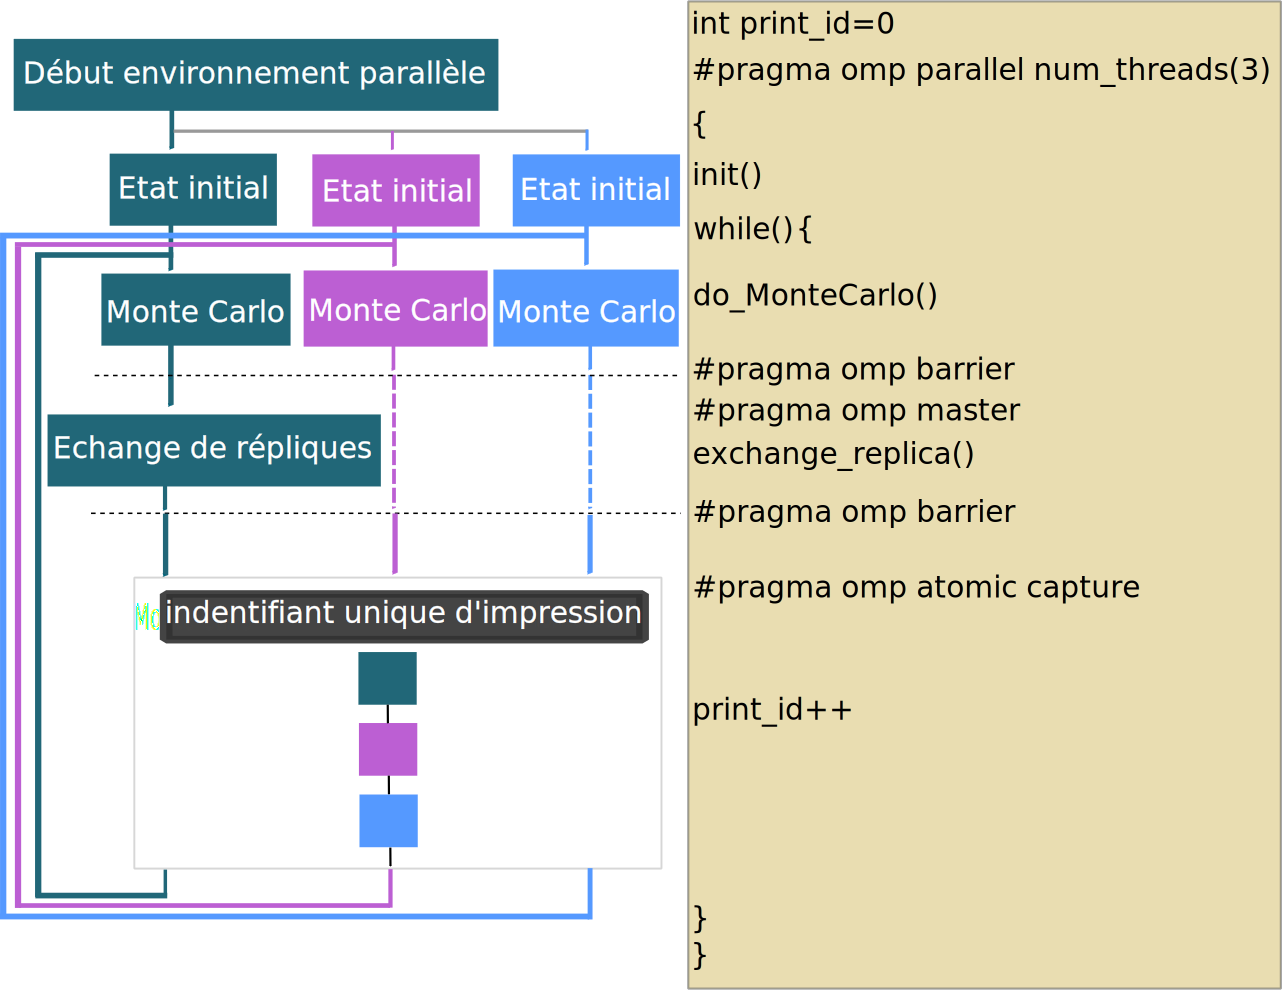
\includegraphics[width=14cm]{figure/openMP.png} 
     \end{tabular}     
     \caption{\textbt{La correspondance entre les directives OpenMP à doite et le conportement des fils d'exécution à gauche sur un REMC simplifié} Sont chématisés, la création d'une région parallèle, deux synchronisations, un région executé uniquement par un fil maître, une affectation séquentielle }
\label{fig:openMP}
   \end{figure}

Pendant l'exécution, le fil d'exécution crée les autres fils. Il possède un statut particulier, il devient le fil maître. Les autres fils se terminent avec la région parallèle; Le maître continue son exécution. Tous les fils ont accès à la même mémoire partagée, notamenent aux variables définis avant la région parrallèle. La déclaration d'une variable dans une région parralèle engemdre la création d'une variable pour chaque fil accessible uniquement par lui. 
   

\subsection{REMC dans proteus}

Comme nous l'avons vu en \ref{REMC} l'algorithme REMC considère plusieurs simulations indépendantes d'un même système. Cela fait de lui un algorithme bien adapté à la programmation parallèle. Deux points demandent une attention particulière l'échange de réplique et la création de l'identifiant unique d'impression, voir \ref{proteusIO}. Le schéma génnéral de REMC dans proteus est présenté à la figure  \ref{fig:openMP}. Une région parallèle est initiée par la directive \og #pragma omp parallel\fg: les différents marcheurs sont créés. Chacuns réalise une trajectoire de type MC jusqu'à un nombre de pas multiple de la période d'échange. A priori l'avancée des marcheurs n'est pas simutanée. Donc une directive \og #pragma omp barrier\fg est placée avant le test d'échange, elle garantie que chacun a effectué le même bon nombre de pas. Une fois tous les marcheurs bloqué par cette directive, ils sont libérés. La directive \og #pragma omp master\fg dédie l'execution du test et de l'échange de réplique au seul marcheur maître. Pour empêché les autres de marcher avant un echange éventuel, une seconde directive \og barrier\fg est placée après les instructions d'échanges. Tout au long d'une trajectoire, des séquences-conformations sont imprimées. Pour facilité le post-traitement, un identifiant unique sur toute l'exécution est attribuée à chacunes. Pour que tous les marcheurs puissent l'incrémenter, l'index qui sert d'identifiant est déclaré comme variable partagée. Pour garantir que chaque passage sur cette instruction retourne une valeur unique une directive \og#pragma omp atomic cpture \fg est utilisée.
 
   \begin{figure}[!htbp]
     \centering
     \begin{tabular}{cc}
       \includegraphics[width=8cm]{figure/re8_Ttraj.png}  &
       \includegraphics[width=8cm]{figure/re8_distri.png}  &
     \end{tabular}     
     \caption{\textbt{}}
\label{fig:PDB}
   \end{figure}
   

\section{affinage de la fonction de test MC}
\section{fonction plus mieux}
\section{constraintes dans les résidues}
\section{Nouveau système de Déplacement}
\section{Print\_threshold}
\section{Label}
\section{allocation variable de la matrice}

\clearpage


%%% Local Variables:
%%% mode: latex
%%% TeX-master: "../these"
%%% End:
